% Format teze zasnovan je na paketu memoir
% http://tug.ctan.org/macros/latex/contrib/memoir/memman.pdf ili
% http://texdoc.net/texmf-dist/doc/latex/memoir/memman.pdf
% 
% Prilikom zadavanja klase memoir, navedenim opcijama se podešava 
% veličina slova (12pt) i jednostrano štampanje (oneside).
% Ove parametre možete menjati samo ako pravite nezvanične verzije
% mastera za privatnu upotrebu (na primer, u b5 varijanti ima smisla 
% smanjiti 
\documentclass[12pt,oneside]{memoir} 

% Paket koji definiše sve specifičnosti master rada Matematičkog fakulteta
\usepackage[latinica]{matfmaster} 
%
% Podrazumevano pismo je ćirilica.
%   Ako koristite pdflatex, a ne xetex, sav latinički tekst na srpskom jeziku
%   treba biti okružen sa \lat{...} ili \begin{latinica}...\end{latinica}.
%
% Opicija [latinica]:
%   ako želite da pišete latiniciom, dodajte opciju "latinica" tj.
%   prethodni paket uključite pomoću: \usepackage[latinica]{matfmaster}.
%   Ako koristite pdflatex, a ne xetex, sav ćirilički tekst treba biti
%   okružen sa \cir{...} ili \begin{cirilica}...\end{cirilica}.
%
% Opcija [biblatex]:
%   ako želite da koristite reference na više jezika i umesto paketa
%   bibtex da koristite BibLaTeX/Biber, dodajte opciju "biblatex" tj.
%   prethodni paket uključite pomoću: \usepackage[biblatex]{matfmaster}
%
% Opcija [b5paper]:
%   ako želite da napravite verziju teze u manjem (b5) formatu, navedite
%   opciju "b5paper", tj. prethodni paket uključite pomoću: 
%   \usepackage[b5paper]{matfmaster}. Tada ima smisla razmisliti o promeni
%   veličine slova (izmenom opcije 12pt na 11pt u \documentclass{memoir}).
%
% Naravno, opcije je moguće kombinovati.
% Npr. \usepackage[b5paper,biblatex]{matfmaster}

% Pomoćni paket koji generiše nasumičan tekst u kojem se javljaju sva slova
% azbuke (nema potrebe koristiti ovo u pravim disertacijama)
\usepackage[latinica]{pangrami}
\usepackage{makecell}
% Datoteka sa literaturom u BibTex tj. BibLaTeX/Biber formatu
%\bib{matfmaster-primer}

% Ime kandidata na srpskom jeziku (u odabranom pismu)
\autor{Jovan Marković}
% Naslov teze na srpskom jeziku (u odabranom pismu)
\naslov{Fino podešavanje jezičkog modela BERT za analizu sentimenta}
% Godina u kojoj je teza predana komisiji
\godina{2025}
% Ime i afilijacija mentora (u odabranom pismu)
\mentor{prof Aleksandar \textsc{Kartelj}, vanredni profesor\\ Univerzitet u Beogradu, Matematički fakultet}
% Ime i afilijacija prvog člana komisije (u odabranom pismu)
\komisijaA{prof Mladen \textsc{Nikolić}, vanredni profesor\\ Univerzitet u Beogradu, Matematički fakultet}
% Ime i afilijacija drugog člana komisije (u odabranom pismu)
\komisijaB{prof Vladimir \textsc{Filipović}, redovan profesor\\ Univerzitet u Beogradu, Matematički fakultet}
% Ime i afilijacija trećeg člana komisije (opciono)
% \komisijaC{}
% Ime i afilijacija četvrtog člana komisije (opciono)
% \komisijaD{}
% Datum odbrane (odkomentarisati narednu liniju i upisati datum odbrane ako je poznat)
% \datumodbrane{}

% Apstrakt na srpskom jeziku (u odabranom pismu)
\apstr{%
Ovaj rad predstavlja različite načine za fino podešavanje velikih jezičkih modela. U radu se analiziraju koncepti velikih jezičkih modela, njihova struktura, osnovne karakteristike i načini na koji se njihova generativna priroda može prilagoditi potrebama za rešavanjem specifičnih zadataka. Kao centralna tema, vrši se analiza primene različitih tehnika finog prilagođavanja modela BERT za rešavanje problema analize sentimenta. Cilj rada je upoređivanje potrebnih resursa i poboljšanja generisanih odgovora prilikom realizacije svake od obrađenih tehnika. 
}

% Ključne reči na srpskom jeziku (u odabranom pismu)
\kljucnereci{veliki jezički modeli, BERT, analiza sentimenta, fino prilagođavanje}

\begin{document}
% ==============================================================================
% Uvodni deo teze
\frontmatter
% ==============================================================================
% Naslovna strana
\naslovna
% Strana sa podacima o mentoru i članovima komisije
\komisija
% Strana sa posvetom (u odabranom pismu)
\posveta{Svim ljudima koje sam upoznao tokom studiranja na fakultetu}
% Strana sa podacima o disertaciji na srpskom jeziku
\apstrakt
% Sadržaj teze
\tableofcontents*

% ==============================================================================
% Glavni deo teze
\mainmatter
% ==============================================================================

% ------------------------------------------------------------------------------
\chapter{Uvod}
% ------------------------------------------------------------------------------
Veštačka inteligencija je pojam koji je učestalo krenuo da se koristi u poslednjoj deceniji, najčešće u kontekstu označavanja prelaska u najnoviji period razvoja nauke i načina svakodnevnog života. Ovaj pojam je, sa druge strane,već dugo poznat u svetu računarskih nauka i njegove tehnike razvijane su još od sredine prošlog veka \cite{AIOrigins}. Iako su dotadašnje primene imale širok spektar različitih problema koji su mogli biti rešavani njima, pažnju svetske javnosti privukao je razvoj jezičkih modela i njihova integracija u svakodnevnom životu. Ovi modeli omogućavaju jednostavnu komunikaciju koja se može odnositi na najrazličitije teme i oblasti. Kada osoba želi da napravi ručak, odradi domaći zadatak, napiše sastav ili pravi plan za teretanu, najčešća putanja vodi do generalizovanih robota koji odgovaraju u sličnom stručnom, prijateljskom ili prilagođenom tonu \cite{LLMUsageSurvey}. 

Ono što omogućava jezićkim modelima da budu efikasni u svom radu je dostupnost velikog broja informacija u svetu. Jezički modeli svoje znanje crpe trenirajući se na milijardama i milijardama najrazličitijih dostupnih podataka iz oblasti života, literature, nauke i kao takvi omogućavaju komunikaciju na gotovo svaku temu koja je korisniku potrebna. Na internetu postoje milioni informacija o receptima za zdrave obroke, načine popravljanja kućnih aparata ili analizama ljudske psihologije, tako da ne čudi što je moguća komunikacija na temu analize osećanja likova u Šekspirovim delima ili istraživanja različitih mogućnosti nastanka univerzuma \cite{DataInAI}.

Međutim, primene ovih modela ne završavaju se samo na rešavanju svakodnevnih zadataka. Njih mogu koristiti i ljudi u obavljanju posebnih specifičnih zadataka, kao što je rad u laboratoriji, pisanje koda ili naučnih radova, u kojima oni postaju eksperti i savetnici iz određenih oblasti. Ova primena razlikuje se od uobičajene zbog svoje uske specijalizovanosti ili manjka dostupnih informacija iz konkretnih oblasti. Takođe, ukoliko želimo da naši modeli ne budu samo mašine u našim očima, već da imitiraju govor pravih ljudi, odgovaraju uvek u nekom specifičnom maniru ili na neki drugi način budu prilagođeni našim potrebama, naophodna je primena posebnih tehnika kojima će se oformljen generalizovan model pretvoriti u specijalizovanog asistenta \cite{LLMCustomization}.

Tehnike koje omogućavaju menjanje ponašanja modela za specifične potrebe nazivaju se tehnikama finog podešavanja (eng. fine-tuning). One obuhvataju spektar različitih metoda za menjanje načina funkcionisanja već istreniranih modela. Mogu se ostvariti na različite načine zahtevajući različite nivoe shvatanja funkcionisanja, kao i strukture pojedinačnih modela. 

Fine-tuning tehnike značajne su zbog toga što cena pravljenja sopstvenih jezičkih modela može biti velika zahtevajući dragocene resurse \cite{CostOfLLMs}. Zbog toga je često praktično izabrati i iskoristiti već postojeće, istrenirane modele i prilagoditi ih sopstvenim potrebama. Na ovaj način zadržavaju se dragocena svojstva odabranih modela, kao što je shvatanje konteksta i mogućnost generalizacije, dok se svojstva modela prilagođavaju specifičnim zadacima. 

Popularnost jezičkih modela ogleda se i u njihovoj širokoj dostupnosti na internetu, kao i konstantnim novim modelima koji se mogu koristiti. Razvijaju se i posebne platforme koje omogućavaju preuzimanje modela, kao što je Hugging Face \cite{Huggingface2023}, koji korisnicima nude postojeća rešenja na koja mogu nadograditi svoje željene funkcionalnosti.

Zbog svoje kompleksne i memorijski zahtevne strukture, promene na modelima mogu oduzeti dragoceno vreme i potrebne resurse ukoliko ih želimo prilagoditi vlastitim potrebama. Ovo je razlog zašto je potrebno istražiti i uporediti različite metode finog prilagođavanja, kako bismo znali koji metod je potrebno primeniti u zavisnosti od dostupnih resursa i potrebnih performansi. 

Moguće je prepoznati različite načine za podelu fine-tuning tehnika, ali ona na kojoj će biti fokus je podela prema broju parametara za treniranje. U ovom slučaju razlikujemo:
\begin{enumerate}
	\item Potpuno fino podešavanje (eng. full fine-tuning) - Svi parametri datog modela mogu se obučavati i menjati svoja unutrašnja stanja.
	\item Parametarski efikasno fino podešavanje (eng. parameter efficient fine-tuning - PEFT)\cite{PEFTArticle} - U ovom slučaju odabira se poskup svih dostupnih parametara modela i na njima su moguće izmene, dok ostali ne menjaju svoja stanja.
\end{enumerate}


U ovom radu biće prikazane sledeće metode finog podešavanja modela:
\begin{enumerate}
	\item potpuno fino podešavanje (eng. full fine-tuning)
	\item fino podešavanje glave za klasifikaciju (eng. classification head fine-tuning) \cite{ClassificationHeadTechnique}
	\item fino podešavanje zasnovano na adapterima (eng. Adapter-based fine-tuning) \cite{AdaptersTechnique}
	\item fino podešavanje zasnovano na matricama niskog ranga (eng. Low Rank Adaptation - LoRA) \cite{LoRATechnique} 
\end{enumerate}

Prvi pristup utiče na celokupnu strukturu modela, dok su ostali pristupi vrste pristupa zasnovanog na parametarski efikasnom finom podešavanju, koji za cilj ima brže i manje zahtevno prilagođavanje modela, koje ne utiče na celokupnu strukturu, već samo na odabrani podskup parametara.

Fino podešavanje glave za klasifikaciju predstavlja jednostavan odabir podskupa parametara za treniranje koji je ograničen samo na poslednji sloj parametara modela. Ideja je da se zadrži većina svojstava već istreniranog modela, kako se ne bi radikalno uticalo na kvalitet modela \cite{BenefitOfClassificationHeadTuning}. Ovaj pristup je koristan u slučaju da su komputacioni i vremenski resursi ograničeni jer se trenira samo mali podskup parametara. Takođe je korisno u slučajevima da se trenira na malom skupu podataka jer su promene izraženije \cite{TuningHeadResources}.

Pristup fine-tuning-a zasnovanog na adapterima podrazumeva umetanje posebnih modula između postojećih slojeva modela. U ovom pristupu zamrzavaju se svi parametri originalnog modela, dok se samo adapteri ostavljaju kao parametri za treniranje. Ovaj pristup donosi sa sobom benefite kao što su:
\begin{enumerate}
\item Komputaciona efikasnost: Mi biramo koliko parametara će biti određeno za treniranje, a najčešće predstavlja oko 1-5\% ukupnog broja parametara modela. 
\item Omogućuje brzu promenu konteksta: Ukoliko postojeće adaptere zamenimo drugim pretreniranim adapterima, omogućuje se brza zamena podešavanja istog modela.
\item Niska cena isporučivanja: Umesto zamene celog modela, dovoljno je isporučiti mali podskup adaptera.
\end{enumerate}
Na ovaj način, adapteri donose mnoge pogodnosti koje su nabrojane uz prilagođavanje samo glave za klasifikaciju, donoseći i benefite u pogledu fleksibilnosti mogučnosti modela.

Nastalo objavljivanjem rada iz 2021. godine, fino prilagođavanje zasnovano na matricama niskog ranga predstavlja jednu od najnovijih metoda fine-tuning-a. U ovom slučaju ubacuju se matrice niskog ranga unutar specifičnih težinskih matrica i tako se samo one podešavaju. Radi po sličnom principu kao i adapteri, tako da sa sobom donosi i sve njihove benefite, ali pažljivo proračunatim izračunavanjima doprinosi još manjem broju parametara za treniranje ( manje od 1\% od ukupnog broja parametara modela ), kao i bržem treniranju.

Iako se tehnike finog podešavanja koje će biti izložene u ovom radu mogu primeniti na sve vrste modela fokus će biti prebačen na Google-ov model BERT, specijalizovan za razumevanje ulaznih podataka, primenjen na poznat problem analize sentimenta \cite{liu2012sentiment}. Kao konkretan primer, biće iskorišćen skup recenzija za sajt IMDB \cite{IMDBDataset} koji se često koristi za potrebe testiranja performansi različitih jezičkih modela.



\chapter{Osnovni koncepti}
\section{Obrada prirodnih jezika}

Obrada prirodnih jezika (eng. Natural Language Processing - NLP) je široka oblast koja je počela da se razvija davno pre pojave velikih jezičkih modela, već oko 30-ih godina prošlog veka \cite{HistoryOfNLP}. U svojoj suštini odnosi se na mašinsko razumevanje teksta napisanog na prirodnom jeziku. Neke od oblasti rada koje ovaj pojam obuhvata su prepoznavanje govora, prevođenje tekstova, sumarizacija teksta itd. Primeri popularnih aplikacija čija suština leži u obradi prirodnih jezika su virtualni asistenti (Alexa, Cortana, Siri...), internet pretraživači, prevodioci, onlajn jezički modeli itd.

Tekst koji se obrađuje može biti struktuiran i nestruktuiran. Primeri nestruktuiranog teksta:
 
\begin{enumerate}
	\item "Milica je pošla u školu."
	\item "Kupi jaja i mleko."
\end{enumerate}

Primeri struktuiranog teksta:

\vspace{1em}
\hspace{2em} \parbox{0.8\linewidth}{%
	\textit{%
		{subjekat: Milica,} \\
		{objekat: škola,} \\
		{radnja: poći}%
	}%
}
\vspace{1em}

ili

\vspace{1em}
\hspace{2em} \parbox{0.8\linewidth}{%
	\textit{%
		<namirnice> \\
		<predmet>jaja</predmet> \\ 
		<predmet>mleko</predmet> \\
		</namirnice>
	}%
}

\vspace{1em}

Struktuiran tekst je lakši za obradu i razumevanje mašinama, međutim ljudima nije prirodno da komuniciraju na ovaj način. Sa druge strane, nestruktuiran tekst je način na koji ljudi komuniciraju, ali je mašinama teško da shvate njegov kontekst i strukturu.

Proces prevođenja nestruktuiranog u struktuiran tekst naziva se shvatanje prirodnih jezika (eng. Natural Language Understanding - NLU) \cite{NLU}, dok se u suptornom smeru primenjuje generisanje prirodnih jezika (eng. Natural Language Generation) \cite{NLG}. 

\section{Veliki Jezički Modeli - LLM}

Unutar široke oblasti obrade prirodnih jezika, koja se tradicionalno fokusira na skup osmišljenih pravila, statističke modele i algoritme fokusirane za izvršavanje pojedinačnih zadataka, razvoj velikih jezičkih modela (eng. Large Language Models - LLMs) predstavljaju značajnu prekretnicu. Za razliku od klasičnih metoda obrade jezika, koje poseduju zasebne načine za procesiranje raznorodnih zadataka, kao što su analiza sentimenta, mašinsko prevođenje itd. jedan dobro istreniran veliki jezički model poseduje mogućnost, kroz generalizaciju i prenos znanja za uspešno korišćenje u sve te svrhe.

LLM-ovi su duboke neuronske mreže, istrenirane na ogromnim količinama tekstualnih podataka (ponekad sadrže i po milijardu tokena). Njihova sadržajnost nije izražena samo na količini podataka iskorišćenih za treniranje, već i u količini parametara koje poseduju , krećuću se od nekoliko stotina miliona ("GPT-2 Small" model poseduje 117 miliona parametara \cite{LLMListHuggingFace}), sve do preko stotina milijardi (Guglov "PaLM" model sadrži oko 540 milijardi parametara \cite{PalmLLM}). Slika 2.1 pokazuje kako se sa razvojem novijih modela eksponencijalno povećava broj parametara za njihovo obučavanje \cite{LLMParameters}. Dalji razvoj modela ide u smeru sve većih i složenijih modela, dok informacije za neke od najnovijih, kao što su GPT-5 \cite{GPT5} i ne otkrivaju njihovu složenost, koja se procenjuje da ima i nekoliko biliona parametara. 

\begin{figure}[!ht]
	\centering
	\label{fig:LLMParametersTimelapse}
	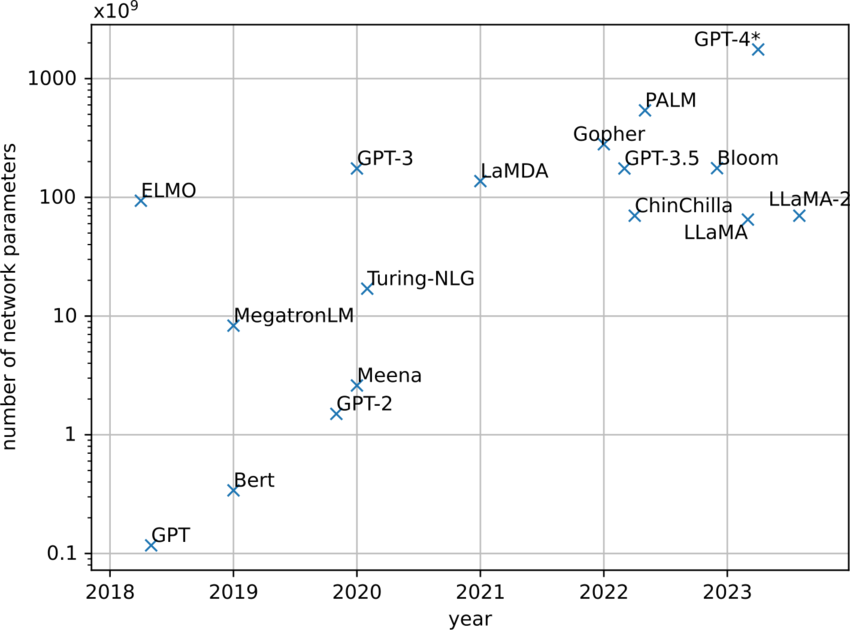
\includegraphics[width=0.7\textwidth]{LLMParametersTimelapse.png}
	\caption{Odnos godine objavljivanja i količine parametara modela, izražen u stotinama milionima. *Broj parametara za GPT-4 nije zvanično objavljen, ali se po procurelim podacima pretpostavlja da je sadrži ok 1760 milijardi parametara.}
\end{figure}

\section{Tokenizatori}
Iako se čini da jezički modeli rade sa sirovim tekstovima podataka, ovo nije tačno. Reči predstavljaju niske slova, odnosno simbola, sa kojima je mašinama teže da rade nego sa brojevima. Zbog toga se unutar modela vrše transformacije rečenica u liste korespodentnih numeričkih vektora kako bi mašinama bio olakšan rad. 

Transformacija ulaznih podataka u vektore koji se prosleđuju modelima naziva se tokenizacija \cite{Tokenization}, a obavlja se pomoću posebnih komponenti koje se nazivaju tokenizatori. Tokenizatori preuzimaju ulazne podatke, vrše njihovu obradu, a na izlaz dostavljaju određen skup tokena. Tokeni mogu biti reči ili delovi reči koji su kodirani na određen način, a zatim su prosleđeni odgovarajučim jezičkim modelima za potrebe treniranja. 

Različiti tokenizatori kodiraju skup reči na različite načine. Prilikom početnog treniranja modela nad ulaznim podacima, način rada tokenizatora može biti značajan za krajnje mogućnosti modela \cite{Huggingface_tokenizers} \cite{Tokenizers}. Zbog različitog načina kodiranja, prilikom rada sa nekim unapred istreniranim jezičkim modelima, bitno je primeniti isti tokenizator, jer u suprotnom može doći do značajnog umanjenja moći modela.

Jedan od najpoznatijih načina za transformisanje reči je kodiranje pomoću parova bajtova (eng. Byte Pair Encoding - BPE) \cite{BPETokenization}. Prvi put je opisan u radu 1994. godine kao jednostavan algoritam kompresovanja podataka \cite{BPEDataCompression}. Prepoznajući njegov značaj, 2016. godine on nalazi svoju primenu pri razvoju jezičkih modela, a zbog svoje jednostavnosti i efikasnosti u mnogima od njih koristi se u originalnoj ili izmenjenoj verziji. Rad ovog algoritma ogleda se u iterativnom pronalaženju učestalih parova bajtova u sekvenci i njihovom objedinjavanju u specijalizovane grupe koje se nazivaju tokenima.

\begin{figure}[!ht]
	\centering
	\label{fig:TokenizationExample}
	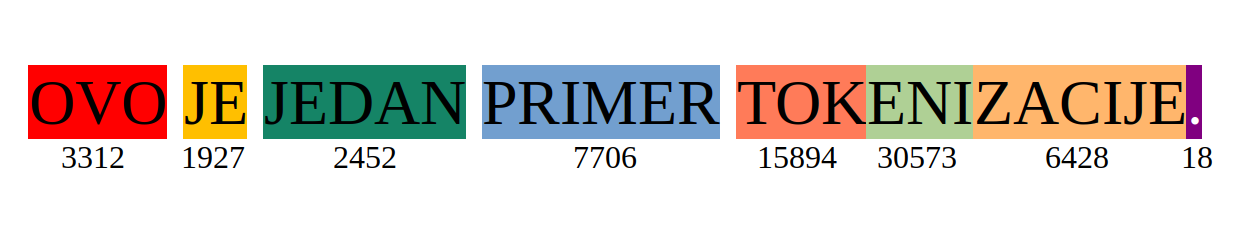
\includegraphics[width=0.9\textwidth]{Tokenization_example.png}
	\caption{Primer rada tokenizatora modela BERTić. Tokeni su označeni različitim bojama, dok je ispod njih njihova brojna vrednost.}
\end{figure}

Na slici 2.2 nalazi se primer rada tokenizatora za model BERTić koji je model posebno napravljen da razume jezik sa naših prostora i sadrži 8 milijardi različitih tokena \cite{BERTic}. 


Kako su tokenizatori programi koji prepoznaju obrasce u tekstu i rečima i dodeljuju im jedinstvene vrednosti na osnovu skupa na kojem su trenirani, moguće je da se desi i da za prosleđen simbol ili reč ne postoji odgovarajući token koji se može generisati. U ovom slučaju tokenizatori vraćaju 
specijalan token koji se naziva nepoznat token (eng. unknown token). Sa svakim neprepoznatim tokenom, gubi se deo informacija, ali ukoliko se ne javlja u velikoj meri, nije potrebno posebno rukovanje u ovim slučajevima.

Pored transformisanja rečenica u niz tokena, tokenizatori takođe imaju i ulogu konvertovanja skupa tokena nazad u rečenice čitljive krajnjim korisnicima.


\section{Transformeri}

Od objavljivanja dokumenta Attention Is All You Need \cite{AttentionIsAllYouNeed}, koji je predstavio istraživački tim iz Google-a 2017. godine, došlo je do značajnog pomaka u razvoju jezičkih modela. Dotadašnji pristupi obrade prirodnog jezika zasnivali su se na rekurentnim neuronskim mrežama (RNN) i modelima duge kratkoročne memorije (LSTM) \cite{RNNAndLSTM}. Ovi pristupi, iako efikasni u hvatanju vremenskih zavisnosti, bili su ograničeni u pogledu paralelizacije i skalabilnosti pri radu sa velikim količinama podataka. Uvođenjem Transformer arhitekture, ovi problemi su u velikoj meri prevaziđeni, a dalji razvoj velikih jezičkih modela (eng. Large Language Models) postao je eksponencijalno brži.

Kako se u dokumentu navodi, Transformeri su sastavljeni od tri vrste gradivnih slojeva koji se nazivaju matrice pažnje (eng. Attention Matrix), neuronske mreže sa propagacijom unapred (eng. Feedforward Neural Network - FNN) kao i normalizacioni sloj (eng. Layer Normalization).
Njihovim naizmeničnim kombinovanjem omogućava se efikasno učenje složenih reprezentacija jezičkih sekvenci. Ključna prednost Transformer arhitekture predstavlja istovremeno obraćanje pažnje na različite delove ulazne sekvence, čime se poboljšava razumevanje konteksta i odnosa između reči \cite{AttentionPaper}. Pored toga, zahvaljujući potpunoj eliminaciji rekurentnih i konvolutivnih struktura, Transformer omogućava visoku paralelizaciju procesa učenja, što ga čini posebno pogodnim za treniranje na savremenim hardverskim arhitekturama \cite{LLMScalingLaws}.

\begin{figure}[!ht]
	\centering
	\label{fig:TransformerExample}
	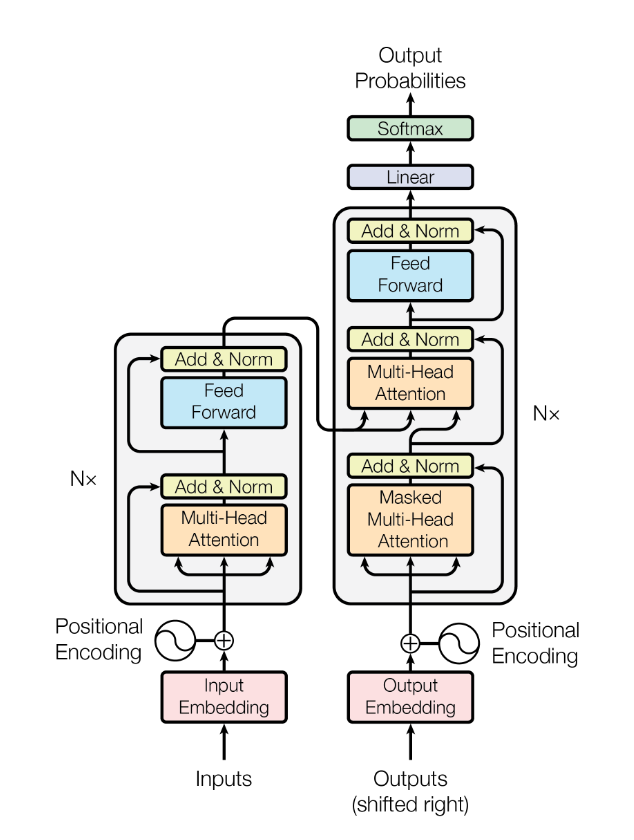
\includegraphics[width=0.9\textwidth]{Transformer_Example.png}
	\caption{Osnovna struktura transformera predstavljena u originalnom radu (Vaswani i drugi). Model se sastoji od enkoder-dekoder arhitekture u kojoj se svaka komponenta gradi od slojeva pažnje (self-attention) i FFN mreža uz rezidualne konekcije i normalizaciju između njih. Dekoder dodatno uključuje cross-attention prema izlazima enkodera.}
\end{figure}

Transformeri nisu ostali ograničeni samo na obradu jezika. Njihova primena se proširila i na druge oblasti mašinskog učenja, poput obrade slika, signala i biomedicinskih podataka, gde su takođe pokazali značajna poboljšanja u performansama u poređenju sa ranijim arhitekturama. Upravo ta univerzalnost i fleksibilnost čine transformatore jednom od najvažnijih inovacija u oblasti veštačke inteligencije poslednje decenije \cite{TransformersForImageRecognition}.

\subsection {Matrice pažnje}

Osnovna uloga ovog sloja je prilagođavanje svake reči određenom kontekstu u kojem se javlja. Iako tokenizator dodeljuje predefinisanu vrednost svakoj reči, ona se dalje transformiše u sloju pažnje u zavisnosti od okruženja u kojem se ta reč nalazi.

Mehanizam pažnje omogućava modelu da za svaku reč identifikuje relevantne informacije iz drugih reči u sekvenci. Intuitivno, to znači da značenje reči ne zavisi samo od njene vrednosti, već i od njenog odnosa prema ostalim rečima u ulaznom tekstu. Veličina dela sekvence koji model može istovremeno da obradi naziva se veličina konteksta (eng. Context size) i ona ima ključan uticaj na performanse modela. Veći kontekst omogućava bogatije reprezentacije, ali istovremeno dovodi do kvadratnog rasta dimenzija matrice pažnje, što značajno povećava računsku složenost.

U zavisnosti od okoline koja se posmatra, razlikujemo:
\begin{enumerate}
	\item Maskirane jezičke modele (eng. Masked Language Models - MLMs), koji posmatraju tokene i sa leve i sa desne strane u posmatranog tokena. Na ovaj način postižu dobre rezultate u zadacima razumevanja jezika i analize teksta. Modeli koji koriste ovu paradigmu su BERT, RoBERTa, ALBERT.
\item Kauzalne jezičke modele (eng. Causal Language Models - CLMs), koji posmatraju isključivo tokene koji prethode trenutnom. Ovi modeli specijalizovani su za zadatke generisanja teksta, a primeri su GPT, LLaMA i Phi modeli.
\item Hibridne modele - koji kombinuju ove dve paradigme, gde ulazna komponenta koristi maskirani pristup, dok izlazna generiše tekst na kauzalan način. Ovaj pristup dovodi do boljih performansi u balansiranim zadacima gde su podjednako bitni i razumevanje i generisanje teksta. Predstavnici su T5 i BART.
\end{enumerate}

Mehanizam pažnje definiše se sledećom formulom:

\begin{equation}
	Attention(Q,K,V) = softmax(\frac{QK^T}{\sqrt{d_k}})V
\end{equation}

Matrica pažnje (eng. Attention Matrix) omogućava modelu da dinamički proceni značaj svake reči u sekvenci u odnosu na ostale reči u kontekstu. Ulazni vektori Q (Query), K (Key) i V (Value) prolaze kroz linearne transformacije koje određuju koliko svaka reč doprinosi reprezentaciji drugih reči. Skalarni proizvod Q\(K^T\) meri sličnost između reči u sekvenci. Što je rezultat veći, to je jača međusobna zavisnost između odgovarajućih reči. Radi numeričke stabilnosti, ubacuje se faktor \(\sqrt{d_K}\)a primenom softmax funkcije dobijaju se verovatnoće koje ponderišu vrednosti vektora V, čime se dobija nova reprezentacija reči koja objedinjuje informacije iz celokupnog konteksta\footnote{Formulom je predstavljena matrica veličine |veličina konteksta| x |veličina konteksta| gde su po kolonama smeštene vrednosti Q (eng. Query), koje predstavljaju rezultat matričnog množenja posebnih podesivih matrica \(M_Q\)(eng. Query Matrix) sa svakom reči u kontekstu, dok su vrednosti K (eng. Key) po redovima nastali množenjem sa drugom matricom \(M_K\) (eng. Key Matrix). Vrednosti u matrici pažnje su skalarni proizvodi koji su blizu 1 ukoliko postoji korespodencija između dve reči. Po svakoj koloni se primenjuje softmax funkcija kako bi se dobile verovatnoće koje konfigurišu u tekstu. Promenljiva T predstavlja temperaturu i obično je u opsegu od 1 do 2, \(\sqrt{d_K}\) 
	pomaže za potrebe stabilnosti prilikom računanja, a predstavlja koren od broja dimenzija vektora K. Svaki od vektora V dobija se kao proizvod posebne prilagodljive matrice \(M_V\) sa vektorima koji predstavljaju reprezentaciju određene reči i u apstraktnom smislu predstavlja vektor koji treba dodati na ostale reči ukoliko želimo da objedinimo njegova svojstva da budu primetna. Nakon primene softmax funkcije, po kolonama se radi još jedan skalarni proizvod sa vektorima V, kako bi se primenio proporcionalni uticaj svake od prethodnih reči. U literaturi, matrica \(M_V\) često je prikazana kao proizvod dve matrice, prva koja preslikava vektor u prostor koji odgovara veličini vektora K i Q, i drugu koja to preslikavanje vraća u originalnu dimenziju. Ova transformacija naziva se i transformacija niskog nivoa (eng. low-rank transformation) }
.

Ova transformacija predstavlja samo jedan od mnogo slojeva koji se paralelno računaju kako bi predložili izmenu u vektoru koji određuje svaku reč. Kada se svi oni sumiraju i dodaju na originalan vektor, dobija se konačna nova vrednost tog vektora. Zbog toga se koristi i pojam višeglave pažnje (eng. Multi Head Attention - MHA) koji prestavlja paralelno izvršavanje više matrica pažnje koje na kraju linearnom transformacijom kombinuje rezultat u konačnu matricu izlaznih vektora, gde svaki red predstavlja konačni vektor određenog tokena.


\subsection{Neuronske mreže sa propagacijom unapred}

Neuronske mreže sa propagacijom unapred predstavljaju jednu od osnovnih arhitektura u oblasti mašinskog učenja i obrade prirodnih jezika \cite{FFN}. Njihova suštinska osobina jeste da se informacije prenose u jednom smeru, od ulaza ka izlazu, bez povratnih veza. U kontekstu transformera, ovaj sloj se može posmatrati kao mesto na kojem se model uči, rezonuje i ubacuje znanje stečeno tokom obuke.  

U okviru transformera, feed-forward slojevi primenjuju se nezavisno nad svakim tokenom, što omogućava visoku paralelizaciju procesa. Tokom transformacije tokena, podaci prolaze kroz više faza: najpre linearno preslikavanje u prostor veće dimenzionalnosti, zatim primenu nelinearne aktivacione funkcije (najčešće ReLU), i konačno vraćanje u izvorni dimenzioni prostor. Prebacivanje u višu dimenzionalnost omogućava modelu da raspolaže većim brojem parametara, čime se otvara prostor za složenije reprezentacije i preciznije zaključivanje.  

Formalno, ovaj postupak opisan je sledećom jednačinom:
\begin{equation}
	FFN(x) = \max(0, xW_{1} + b_{1})W_{2} + b_{2}
\end{equation}

\textit{U ovoj formuli \(W_{1}\) i \(W_{2}\) označavaju matrice težina, \(b_{1}\) i \(b_{2}\) vektore slobodnih članova tih matrica, dok funkcija max() predstavlja ReLU\cite{ReLU} aktivaciona funkcija.}

U praksi se, pored ReLU funkcije, koriste i varijacije poput GeLU\cite{GeLU} ili Swish\cite{Swish} koje omogućavaju stabilnije gradijente i bolje performanse u određenim zadacima. Takođe, dimenzije matrica \(W_1\) i \(W_2\) određuju kapacitet modela - veće dimenzije omogućavaju veću moć rezonovanja, ali po cenu veće računske složenosti i veće mogućnosti preprilagođavanja. Ove karakteristike čine FFN sloj veoma fleksibilnim, omogućavajuću da se njegovo ponašanje adaptira pažljivim izborom parametara i aktivacione funkcije.

\subsection { Normalizacioni sloj }

Normalizacioni sloj je komponenta u transformeru čija je uloga stabilizacija i ubrzavanje procesa treniranja. Oni se postavljaju između slojeva pažnje i neuronskih mreža i primenjuje se po pojedinačnom tokenu normalizujući njegov vektor. Na ovaj način se ublažava problem nestajućih i eksplodirajućih gradijenata i doprinosi stabilnijem treniranju modela.

U originalnom radu, izlaz ovog sloja se opisuje formulom:

\begin{equation}
LayerNorm(x + Sublayer(x))
\end{equation}

\textit{Ovde Sublayer() predstavlja funkciju koja vrši transformacije nad bilo kojem od transformacionih slojeva (matrica pažnje ili nauronske mreže sa propagacijom unapred).}

Ovaj pristup je poznat kao \textit{Post-LayerNorm} i u njemu se proces normalizacije izvršava nakon sabiranja rezultata sa početnim vektorom. Nasuprot ovome, noviji modeli često koriste \textit{Pre-LayerNorm} varijantu u kojoj se normalizacija vrši pre početka obrade podataka.

\begin{equation}
	X+Sublayer(LayerNorm(X))
\end{equation}

Ovaj pristup se pokazao stabilnijim kod veoma dubokih transformera i omogućava bolju propagaciju gradijenata \cite{LayerNorm}.


\vspace{1cm}
Svi predloženi slojevi međusobno se smenjuju i u svakoj iteraciji približavaju cilju. Matrice pažnje služe za međusobno shvatanje odnosa između povezanih struktura i time njihovo prilagođavanje kontekstu u kojem se javljaju. Nasuprot tome, prolazak tokena kroz neuronsku mrežu obavlja se samostalno i nezavisno od okoline, gde se primenjuje stečeno znanje modela. Normalizacioni slojevi su postavljeni između njih kao konfiguracioni slojevi koji osiguravaju stabilna i brza izračunavanja. U svakom transformeru ova tri sloja se međusobno smenjuju i ponavljaju nekoliko desetina ili stotina puta, čime se obezbeđuje mogućnost učenja složenih jezičkih i semantičkih obrazaca.   

\section {BERT model}
Model BERT\cite{BertModel} nastao je 2018. godine od strane stručnjaka iz Guglovog tima. Motivacija za razvoj ovog modela bilo je zapažanje da su dotadašnji modeli koristili isključivo čitanje konteksta sa leve ili sa desne strane. Ovaj model, čije puno ime stavlja akcenat upravo na njegovu karakteristiku da pri analizi rečenica koristi kontekst i sa leve i sa desne strane (eng BERT - Bidirectional Encoder Representations from Transformer), pomerio je granice mogućnosti rezonovanja modela. 

Unidirekcioni modeli (oni koji koriste samo kontekst sa leve ili sa desne strane svake reči) pokazuju se dobro na zadacima generisanja teksta, međutim često se javljaju sub-optimalna rešenja usled toga što se ne uzima u obzir kontekst iz cele okoline, već samo sa jedne strane teksta. Sa druge strane, za potrebe razumevanja celokupnog konteksta, bidirekcioni modeli se pokazuju kao bolji izbor. U ove probleme spadaju klasifikacija teksta, odgovaranje na pitanja ili analiza sentimenta.

Bidirekciona priroda BERT modela omogućava jedinstven način treniranja modela, optimizovanjem MLM (Masked Language Model) funkcije cilja. Ovo se postiže tako što MLM nasumično maskira tokene sa ulaza, a cilj je da se pomoću konteksta uspešno izvrši predikcija maskiranih tokena. Istovremenim spajanjem konteksta sa obe strane, ovaj model naziva se i dubokim bidirekcionim modelom, nasuprot plitkih bidirekcionih modela, nalik na ELMo\cite{ELMo} model koji koristi konkatenaciju dva odvojena unidirekciona sloja.

Drugi zadatak na kojem se BERT model trenirao je predviđanje sledeće rečenice (eng. Next Sentence Prediction - NSP). Ovo je zadatak binarne klasifikacije u kojoj model uči da prepozna da li druga rečenica logički sledi nakon prve. Ovaj zadatak od suštinskog je značaja za razumevanje odnosa među rečenicama u širem tekstu.

Što se tiče unutrašnje strukture, osnovni BERT model sastoji se od 12 slojeva transformera (svaki uključuje mehanizam višeglave pažnje, feed-forward mrežu i normalizaciju), pri čemu se svaki token reprezentuje kao vektor dimenzije 768. Vokabular modela obuhvata oko 30 000 tokena, a ukupno broj parametara iznosi približno 110 miliona\footnote{Od ukupno 110 miliona parametara u modelu, oko 23 miliona koristi se u embedding slojevima, dok MHA i FFN koriste respektivno približno 2.3 i 4.7 miliona parametara po svakom od 12 slojeva. Ovde posttoje i positional embedding slojevi, kao i slojevi normalizacije, ali njihov doprinos je zanemarljiv u ovoj računici }.


Model je treniran na ogromnim tekstualnim korpusima sa ciljem da obuhvati što širi spektar jezičkih stilova i domena. Konkretno, korišćen je BookCorpus skup podataka koji sadrži oko 800 miliona reči iz više od 11 000 knjiga različitih žanrova, kao i engleska verzija Vikipedije koja obuhvata oko 2.5 milijarde reči iz više od 2.5 miliona članaka.


\section{Problem analize sentimenta}

Problem analize sentimenta (eng. Sentiment analysis) predstavlja zadatak klasifikacije teksta u kojima je cilj odrediti da li odražava pozitivno ili negativno mišljenje o nekoj temi. Zbog svoje jednostavnosti za shvatanje, velike količine skupova podataka koja se može pronaći iz različitih oblasti, kao i različitih mogućnosti za generisanje cilja, ovaj problem predstavlja jedan od najosnovnijih koji se koriste u svrhu testiranja rezonovanja jezičkih modela. Skupovi tekstova mogu poticati iz različitih izvora, kao što su internet forumi, ocene proizvoda poručenih preko interneta, komentari na društvenim mrežava, ocene filmova... Kao cilj klasifikacije česte su podele na dve (pozitivno ili negativno) ili  tri (pozitivno, negativno ili neutralno) klase, a moguće je i na izlazu generisati brojčanu vrednost (na primer ocena od 1 do 10, gde 1 predstavlja najlošiju ocenu, a 10 najbolju).

Modeli specijalizovani za rešavanje problema analize sentimenta svoju primenu mogu takođe naći na različitim mestima. Značajni mogu biti u sistemima preporuke gde se koriste informacije o utiscima  proizvoda, ali takođe i na društvenim mrežama gde se prati koliku reputaciju imaju određeni brendovi ili organizacije. Omogućavaju praćenje uspešnosti filmova/serija, ali i političkih kampanja ili događaja u svetu. Takođe bitna stavka je i korišćenje za potrebe ispitivanja finansijskih tržišta, gde je bitno prepoznati mogući uspeh nekog proizvoda u ranoj dobi. Pored nabrojanih, postoje i razne druge oblasti \cite{SentimentAnalysisApplication}.

Zbog svoje raznovrsnosti, kako granulacije na kojoj se analiza može vršiti (analiza dokumenata, pasusa, rečenica, komentara...)\cite{SentimentAnalysisGranularity}, tako i kompleksnosti samih tekstova (analiza emoji-ja, lokalizama, formalan ili neformalan govor, reči u kojima su sva slova velika, sarkazma u tekstu...) u ovim problemima mogu se javljati razni izazovi koje modeli treba uspešno da prevaziđu \cite{SentimentAnalysisChallenges}.

Analiza sentimenta jedna je od starijih problema u oblasti klasifikacije, i za njeno rešavanje mogu se koristiti mnoge metode, kao što su klasične metode nalik na Naivni Bajes\cite{SANaiveBayes} ili sistem potpornih vektora\cite{SASVM}, metode dubokog učenja nalik na konvolutivne\cite{SAConvolutional} ili rekurentne neuronske mreže\cite{SARecurrent}, LSTM (Long-short term memory)\cite{SALSTM}... a moguće je i koristiti jezičke modele zasnovane na transformerima, kao što su BERT, DistilBERT, RoBERTa...

Trenutno je dostupan veliki broj različitih skupova za probleme analize sentimenta, a neki od najpoznatijih su SST (Stanford Sentiment Treebank)\cite{SSTDataset}, Amazon products review \cite{AmazonDataset}, Sentiment140 \cite{Sentiment140Dataset}, IMDB Large Movie Review Dataset \cite{IMDBDataset} i drugi.


\subsection{Large Movie Review Dataset}
Large Movie Review Dataset je skup podataka nastao sastavljen od recenzija filmova sa sajta IMDB (Internet Movie Database). Nastao je 2011. godine, a kreirao ga je Andrew L. Maas \cite{IMDBDataset}. On sadrži ukupno 50 000 recenzija, ravnomerno podeljenih na pozitivne i negativne, što ga čini pogodnim za zadatke binarne klasifikacije sentimenta.

Svaka recenzija je označena kao pozitivna ili negativna na osnovu ocene filma dodeljene od strane korisnika. Recenzije sa ocenom 7 ili više smatraju se pozitivnim, dok se recenzije sa ocenom 4 ili manje smatraju negativnim. Recenzije sa osrednjim ocenama (5 i 6) su izostavljene kako bi klasifikacija bila jasna i binarna.

Ovako transformisane, recenzije su ravnomerno organizovane u trening i test skupove bez preklapanja, kako bi se smanjila pristrasnost prema nekoj od klasa, dok veličina skupa omogućava treniranje savremenih jezičkih modela.


\chapter{Fino podešavanje velikih jezičkih modela}
Fino podešavanje nastaje prilagođavanjem pre-treniranog modela kao osnove na manjem domenski-određenom skupu. Ono što razlikuje ovu metodu od klasičnog treniranja modela, jeste to što se kao osnova koristi model koji već ima opsežno znanje i percepciju lingvističkih pojmova i njihovih odnosa. Zbog toga, fino podešavanje predstavlja dodatni korak koji može značajno doprineti rezultatima izvršavanja modela u oblastima za koje je dodatno treniran.

\section{Značaj i uloga finog podešavanja}
Fino podešavanje nadograđuje postojeće znanje modela, prilagođava ga oblasti u kojoj se očekuje njegovo korišćenje, poboljšavajući performanse dok istovremeno koristi manje kompjuterskih resursa ili podataka pri njihovoj obradi. Zbog svega ovoga, primena finog podešavanja postala je popularna u NLP zadacima, pogotovo u oblasti klasifikacije teksta, analize sentimenta i generisanja odgovora. 

Pogodnosti korišćenja finog podešavanja, ukoliko je ono moguće, su brojne, a neke od njih su date u nastavku:

\begin{description}
	\item[$\bullet$ Prenos znanja (eng. Transfer Learning)] Fino podešavanje omogućava modelu da zadrži svoje stečeno generalno znanje i dalje ga prilagodi specifičnim zadacima. Ovaj proces značajno smanjuje vreme i resurse u odnosu na treniranje modela od starta, kako model već poseduje snažne osnove u shvatanju prirodnih jezika \cite{howard-ruder-2018-universal}. 
	\item[$\bullet$ Smanjena  količina potrebnih podataka] Kako pre-trenirani modeli već poseduju izvesnu količinu znanja, fino podešavanje je usmereno većinom ka shvatanju suptilnijih veza između relevantnih pojmova u definisanom domenu, nije potrebna velika količina podataka za njegovo prilagođavanje. Ovo je naročito korisno u specijalizovanim oblastima gde ne postoje veliki označeni skupovi ili u primeni na jezike za koje ne postoje ekstenzivni resursi\cite{peters-etal-2018-deep}.  
	\item[$\bullet$ Poboljšana generalizacija] Kako fino podešavanje obično obohvata prilagođavanje samo pojedinih elemenata modela, umesto svih elemenata što je slučaj kod inicijalnog treniranja, na ovaj način može se zadržati visok stepen generalizacije početnog modela, smanjujući mogućnost za preprilagođavanjem modela \cite{brown2020languagemodelsfewshotlearners}.	
	\item[$\bullet$ Efikasna isporuka modela] Fino podešeni modeli računski su efikasniji za primenu u aplikacijama u stvarnom svetu, kako ne zahtevaju pre-treniranje u punom obimu. Ovo ih čini podesnim za isporuku u produkcionim okruženjima gde resursi mogu biti ograničeni. Dodatno, fino podešavanje omogućava prilagođavanje modela bez potrebe za potpuno novom arhitekturom.
	\item[$\bullet$ Prilagođavanje na različite zadatke] Fino podešeni modeli omogućavaju jednom pre-treniranom modelu da se prilagodi na širok spektar NLP zadataka. Umesto da postoji poseban model za svaki zadatak, fino podešenim modeli može se promeniti svrha bez ekstenzivnih modifikacija.	
	\item[$\bullet$ Performanse u domenskim zadacima] Fino podešavanje omogućava modelima visoke performanse u specijalizovanim oblastima, nalik na biomedicinu, pravo ili finansije, kao i na nove i nedovoljno dokumentovane oblasti. Ukoliko pre-treniran model posveti pažnju domenski specifičnim podacima, on može naučiti posebne žargone i pojmove i njihove odnose i kasnije ih primeniti u praksi\cite{BioBERT}.
	\item[$\bullet$ Brža konvergencija] Kako je pre-treniran model već prilagođen generalnom shvatanju jezika, dodatne izmene konvergiraju brže nego kod modela koji sve moraju da preračunaju ispočetka. Ovo rezultuje manjem vremenu treniranja kao i manjim računskim zahtevima, što omogućava brže eksperimentisanje sa različitim tehnikama finog podešavanja i čini ga preferiranim metodom za mnoge primene NLP-a u stvarnom svetu.

\end{description}

\section{Vrste finog podešavanja}
Kako fino podešavanje predstavlja opšti način za usmeravanje modela ka specifičnim oblastima za koje će biti korišćen, njegovo izvršavanje može se ostvariti na različite načine. U opštem smislu, metode korišćene u svrhu finog podešavanje mogu se implementirati imajući u vidu 3 različita pristupa:
\begin{description}
	\item[$\bullet$ Po podacima koji se koriste] 
	\item[$\bullet$ Po broju datih primera] 
	\item[$\bullet$ Po strategiji odabira parametara koji se modifikuju] 
\end{description}

\subsubsection{1. Po podacima koji se koriste}
U ovoj podeli vrši se fino podešavanje modela kroz različite pružene podatke a najčešće zavisi od problema koji se rešavaju. 
\begin{itemize}
	\item \textbf{Nadgledano fino podešavanje} – Model je treniran nad labelisanim skupom, kako bi dodatno prilagodio svoje parametre. Korisno za rešavanje problema klasifikacije ili mašinske prevođenja teksta. 
	\item \textbf{Nenadgledano fino podešavanje} – Model se trenira na neoznačenim podacima u svrhu daljeg shvatanja veza između elemenata teksta. Korisno ukoliko model želimo da upoznamo sa usko specifičnim oblastima ili oblastima za koje nema puno podataka. 
	\item \textbf{Fino podešavanje kroz prompt instrukcije} – Umesto modifikacije parametara modela, modelu se nagoveštava način na koji treba da generiše odgovor. Korisno ukoliko nam je struktura ili veličina generisanog odgovora bitna.
\end{itemize}

\subsubsection{2. Po broju datih primera}
U ovom slučaju kao značajna komponenta figuriše količina pruženih podataka. Ukoliko imamo ograničen skup podataka, i treniranje na svega nekoliko pruženih instanci može poboljšati performanse modela.
\begin{enumerate}
	\item \textbf{Učenje bez primera (eng. Zero-shot learning)} – U ovom slučaju model se izvršava bez ikakvog predznanja o specifičnostima za zadatu oblast, oslanjajući se na svoje pre-trenirano znanje.
	\item \textbf{Učenje sa malo primera (eng. Few-shot learning)} – U ovom slučaju modelu ja pružen mali skup označenih podataka (često svega 2-3 primera), najčešće u svrhu uspešne generalizacije problema.
	\item \textbf{Puno fino podešavanje} – Model se trenira na velikom skupu kako bi se potpuno prilagodio postavljenim zadacima.
\end{enumerate}

\subsubsection{3. Po strategiji odabira parametara koji se modifikuju}
U zavisnosti od odabrane strategije, kao i količine parametara kojima je omogućeno treniranje može se balansirati između prilagodljivosti modela specifičnim zadacima kao i zadržavanju generalizovanog znanja koje model poseduje. Ovo je oblast finog podešavanja koja poseduje najveće mogućnosti i mnogo različitih načina za ostvarivanje. Zbog toga će se u ovom radu najviše pažnje posvetiti upravo ovim metodama finog podešavanja i ispitati njihov uticaj na model.
\begin{itemize}
	\item \textbf{Potpuno fino podešavanje (eng. Full Fine-Tuning)} – Svi parametri modela označavaju se kao mogući za treniranje. Ovaj pristup zahteva najviše računskog vremena kako utiče na celokupan model.
	\item \textbf{Parametarski efikasno fino podešavanje (eng. PEFT - Parameter-Efficient Fine-Tuning)} – 
	Širok spektar različitih strategija za fino podešavanje, u opšem smislu odnose se na zamrzavanje velikog broja parametara modela, dok se za treniranje koristi manji broj postojećih ili dodatih parametara kako bi se ubrzao proces treniranja i prilagodio model bez gubitka moći generalizacije. U ovu kategoriju potpadaju mnogi pristupi, od kojih su najpoznatiji:
	\begin{itemize}
			\item \textbf{Fino podešavanje zasnovano na adapterima (eng. Adapter-based fine-tuning)} – Modelu se svi parametri označavaju kao netrenirajući, a ubacuje se dodatni sloj adaptera koji se prilagođava. Na ovaj način smanjuju se računski zahtevi, a dosta prostora se ostavlja eksperimentisanju sa slojevima adaptera i njihovog uticaja na specifične probleme.
			\item \textbf{Fino podešavanje zasnovano na matricama niskog ranga (eng. Low-Rank Adaptation)} – Popularan efikasan metod koji smanjuje korišćenje memorije trenirajući podskup težinskih matrica.
	\end{itemize}	
	
\end{itemize}

Neki pristupi finom podešavanju kombinuju različite nabrojane tehnike kako bi maksimalno iskoristili mogućnosti svojih modela. Odabir korišćene tehnike pre svega zavisi od problema koji se rešava, dostupnih kompjuterskih resursa i količine dostupnih podataka, kao i poznavanja unutrašnje strukture različitih modela.


\section {Potpuno fino podešavanje}
Potpuno fino podešavanje (eng. Full Fine Tuning) predstavlja najklasičniji i najdirektniji pristup prilagođavanju velikih jezičkih modela specifičnom zadatku. Suština ove metode je da se svi parametri modela treniraju ponovo na ciljanom skupu podataka, vršeći potpunu optimizaciju težina mreže, nasuprot dodavanju ili modifikaciji specifičnih slojeva. Na ovaj način, model se u potpunosti prilagođava karakteristikama novog zadatka, jer svaka njegova sastavna komponenta prolazi kroz dodatni proces učenja\cite{radford2019language}.

Jedna od najvećih prednosti full fine-tuninga je ostvarivanje visokih performansi. Pošto se svi parametri optimizuju, model ima potencijal da postigne vrhunske rezultate u ciljanom zadatku, naročito kada ima dovoljno veliki i reprezentativan skup podataka na raspolaganju. Ukoliko je potrebno da se model prilagodi specifičnoj oblasti rada i terminologiji, kao što je medicinska ili pravna dokumentacija, gde je takođe dostupan veliki broj informacija, ovo je često preporučen pristup \cite{christophe2024med42evaluatingfinetuning}. 

Glavni izazov kod ovog pristupa je računska složenost. Prilagođavanje milijardi parametara zahteva ogromne resurse, kako u smislu GPU memorije, tako i u vremenu treniranja. Pored toga, koristi se i značajna memorija, jer svaka verzija prilagođenog modela zauzima jednak prostor kao i originalni model. Zbog sve većeg broj parametara koje savremeni modeli poseduju, ovaj pristup postaje sve teži za praktično ostvarivanje i često nije održiv za modele koji imaju preko nekoliko milijardi parametara. 

Drugi značajni problemi prilikom potpunog finog podešavanja predstavljaju mogućnost overfittinga i nestabilnog treniranja. Kada se trenira ceo model, ukoliko je količina podataka u ciljnim domenima mala, model može da nauči napamet trening skup umesto da generalizuje znanje. Sa druge strane, količina i vrsta podataka koja se pruža modelu takođe može značajno doprineti različitim performansama modela. Jedna studija istraživača sa Saarland i EPFL univerziteta ukazala je da prilikom full fine-tuninga ponašanje modela može značajno varirati, čak i pri istim hiperparametrima zbog problema u optimizaciji (npr. nestajući gradijenti) i nepredvidivih razlika u generalizaciji iz istih gubitaka. Ovo znači da čak i redosled i izbor primera mogu direktno uticati na stabilnost i konačne performanse modela \cite{mosbach2021stabilityfinetuningbert}.

Obzirom na to da se prilikom treniranja na ovakav način menja celokupna struktura modela, posebno je potrebno obratiti pažnju na parametar stope učenja koji se koristi.
Jedan od najkarakterističnijih problema koji se mogu javiti u procesu potpunog prilagođavanja je katastrofalno zaboravljanje. Ovo je pojava u kojoj inicijalne težine modela gube svoja mogućnost generalizacije. Da bi se ovo sprečilo, za stopu učenja se  postavlja vrednost daleko manja od one korišćene u inicijalnom procesu treniranja modela \cite{zhai2023catastrophicforgetting}.

U poređenju sa alternativnim metodama, full fine-tuning se posmatra kao zlatni standard kada resursi nisu ograničeni. Iako je njegova praktična primena ograničena na istraživačke institucije ili kompanije sa snažnim hardverskim infrastrukturama i obimnom količinom podataka, ovaj pristup često se koristi kao referentna tačka u odnosu na nove metode koje teže da postignu slične rezultate uz značajno manju potrošnju resursa. 

\section {Fino podešavanje klasifikacione glave}
Nasuprot potpunom finom podešavanju, fino podešavanje klasifikacione glame zamrzava veliku većinu slojeva ostavljajući samo mali podskup parametara koji se nalaze u poslednjem sloju podložnim za treniranje. Ideja iza ovog pristupa je da se očuvaju bogate postojeće reprezentacije jezika koje model već poseduje \cite{BertModel}.

Ovaj pristup rešava većinu glavnih problema potpunog finog podešavanja, jer drastično smanjenje broja parametara za optimizaciju vodi značajnim uštedama. Ubrzava proces treniranja i smanjuje potrošnja energije. Potrošnja memorije za pravljenje različitih verzija modela primetno je manja jer je samo potrebno preneti modifikovan poslednji sloj modela. Pošto se jezgro modela ne menja, značajno se i smanjuje rizik od problema katastrofalnog zaboravljanja. Prednost se ogleda i u stabilnosti treniranja, jer je treniranje malih slojeva numerički stabilnije i manje podložno problemima optimizacije\cite{mosbach2021stabilityfinetuningbert}. Potreban broj primera da bi se izbeglo preprilagođavanje takođe je manji zbog malog skupa parametara koji se menjaju.

Glavna ograničenja fine-tuninga klasifikacione glave je njegova ograničena primena. Ukoliko je potrebno sveobuhvatno prilagođavanje specifičnom zadatku, čiji domen podataka značajno odstupa od onoga na čemu je model treniran, performanse mogu biti suboptimalne. Odavde se zaključuje da je u ovom pristupu značajan i izbor modela nad kojim će se prilagođavanje ostvarivati, jer osnovno shvatanje konteksta ostaje nepromenjeno.

U praksi ovaj pristup se često koristi za klasifikacione zadatke poput analize sentimenta, kategorizacije teksta ili detekcije namere. Takođe je koristan u scenarijima kada su skup za treniranje, računski, vremenski ili memorijski resursi ograničeni. U ovakvim specifičnim situacijama, izborom ove tehnike prilagođavanja postiže solidan nivo performansi \cite{zaken2022bitfitspeft}. 

\section {Fino podešavanje zasnovano na adapterima}
Adapteri predstavljaju jednu od najznačajnijih tehnika parametarski efikasnog prilagođavanja jezičkih modela. Oni uvode male dodatne neuralne module - adapterske slojeve (eng. Adapter layers) unutar već postojećih (npr. između feed-forward slojeva u transformeru), pri čemu se samo oni treniraju, dok originalna mreža ostaje nepromenjena. Ovime se ostvaruje kompromis između potpunog fine-tuninga i prilagođavanja samo klasifikacione glave \cite{AdaptersTechnique}.

Tipična arhitektura adaptera uključuje takozvanu "usko grlo" arhitekturu (eng. bottleneck architecture), pri kojoj se ulazni vektor projektuje u prostor manje dimenzionalnosti, prolazi kroz nelinearnu transformaciju i vraća nazad u originalan prostor. Formula koja ovo opisuje je:
\begin{equation}
	f_{adapter}(x) = W_{up}g(W_{down}x + b_{down}) + b_{up},
\end{equation}
gde su
\begin{description}
	\item \(W_{down} \in R^{r \times d}\) - matrica koja preslikava originalnu dimenzionalnost u manju (r << d), praveći "usko grlo"
	\item \(W_{up} \in R^{d \times r}\) - matrica koja vraća vektor iz niže dimenzionalnost u originalan prostor
	\item \(g(\dot)\) - nelinearna funkcija (najčešće ReLU) 
	\item \(b_{down}\) - vektor pomeraja (bias) unutrašnje dimenzije r
	\item \(b_{up}\) - vektor pomeraja originalne dimenzije d 
\end{description} 

Ovako definisan modul ubacuje se u model uz rezidualnu konekciju
\begin{equation}
	h_{out} = x + f_{adapter}x
\end{equation}

Ova redukcija smanjuje broj parametara koje je potrebno trenirati na samo \( W_{up}, W_{down}, b_{up} i b_{down}\), što predstavlja \(O(d \dot r)\) parametara za treniranje, omogućavajući efikasno učenje specifičnih karakteristika zadatka. Primer arhitekture dat je na slici 3.1, a preuzet je iz rada Parameter-Efficient Transfer Learning for {NLP}\cite{AdaptersTechnique}.

\begin{figure}[!ht]
	\centering
	\label{fig:AdaptersExample}
	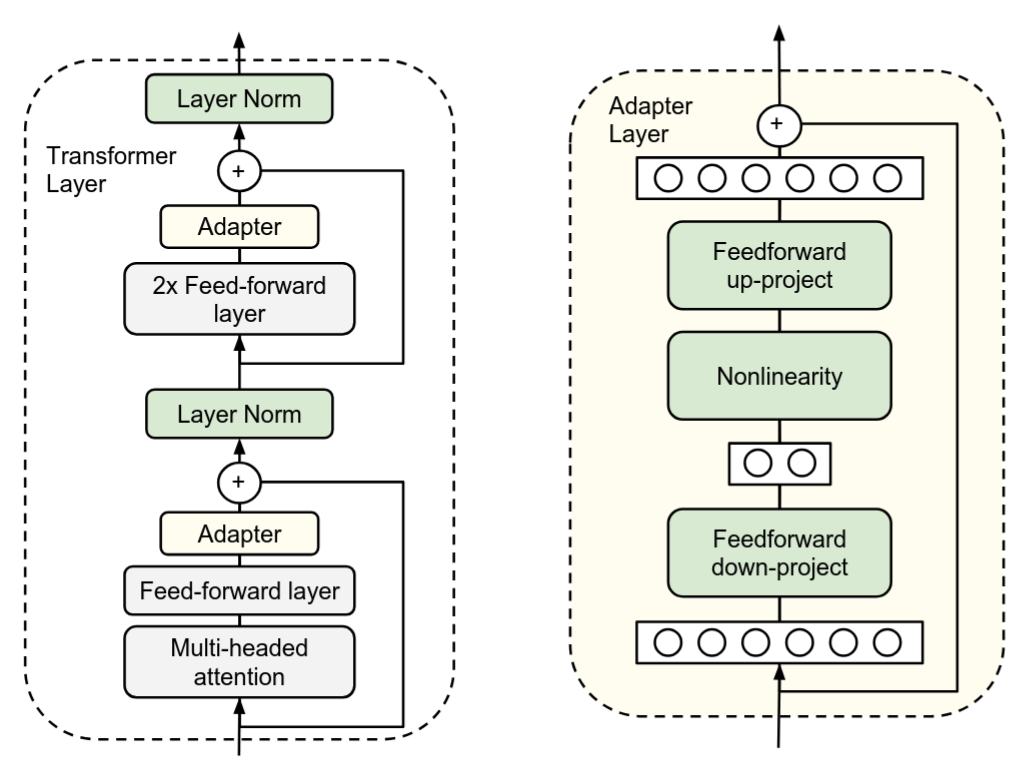
\includegraphics[width=0.9\textwidth]{Adapters_Example.png}
	\caption{Primer arhitekture zasnovanog na adapterima. Feedforward up/down-project predstavljaju funkcije koje vektor preslikavaju u prostor više/niže dimenzionalnosti. }
\end{figure}

Implementacija adaptera u modelima najčešće je ostvarena kroz ubacivanje modula u dve tačke unutar svakog BERT transformer sloja: nakon self-attention izlaza i nakon feedforward izlaza. Ovo predstavlja implementaciju originalne Houlsby \cite{AdaptersTechnique} arhitekture. Alternativni pristup je predložen od strane Pfeiffer-a \cite{pfeiffer2020adapterapplications} koji sugeriše dodavanje adaptera samo nakon attention sloja, kako bi se napravila dodatna ušteda parametara za treniranje, dok su eksperimenti pokazali da se pri tome ne gubi značajno na preciznosti. 

Osnovna prednost ovog pristupa je parametarska i memorijska efikasnost. Kod adaptera dovoljno je čuvanje samo parametara dodatnih slojeva, čime se troškovi skladištenja i isporučivanja drastično smanjuju. Takođe, dodavanje malih modula, specifičnih za određene zadatke čine ih pogodnim za scenarije sa više zadataka ili domena, čineći ih fleksibilnijim u odnosu na samo prilagođavanje klasifikacione glave.

Modularnost adaptera posebno ih čini podobnim za korišćenje za rešavanje različitih raznorodnih familija problema, pri čemu je dovoljno zameniti adaptere specijalizovane za svaki zadatak. Ovime se omogućava ponovno korišćenje istog osnovnog modela, nasuprot pravljenju i dostavljanju pojedinačnih za svaki zadatak \cite{bapna2019adapteradaptation}.

Kao i kod prilagođavanja samo klasifikacione glave, i ovde na kvalitet utiče sam osnovni model koji se koristi. Sposobnost adaptera da se prilagode zadacima imaju svoja ograničenja i mogu zaostajati za full fine-tuningom kada je reč o prilagođavanju za ekstremno specifične zadatke. Takođe, sama struktura adaptera i njihovo pozicioniranje u osnovnom modelu može predstavljati iscrpan proces u kojem rezultati mogu značajno varirati \cite{he2021adaptereffectiveness}.

Primena adaptera naročito dolazi do izražaja u industrijskim aplikacijama gde je potrebno održavati veliki broj modela za različite klijente ili jezike. Ovaj pristup u tim situacijama vodi velikom smanjenju troškova održavanja, nasuprot održavanju velikog broja različitih modela. Kao relativno nov pristup učenju modela, ostavlja prostora za dodatna istraživanja u cilju daljih poboljšanja performansi modela \cite{pfeiffer2020adapterapplications}.


\section {Fino podešavanje zasnovano na matricama niskog ranga}
Nastalo radom objavljenom 2021. godine od strane Edward Hu i Yelong Shen-a, fino podešavanje zasnovano na matricama niskog ranga (eng. Low-Rank Adaptation - LoRA) predstavlja osnovu novog state-of-the-art načina za fino prilagođavanje modela \cite{LoRATechnique}. U ovom pristupu polazi se od zapažanja da se umesto direktnog menjanja težina modela zapravo prate promene koje želimo da primenimo na matričnom nivou. Dakle, uz svaku matricu koju želimo da treniramo možemo dodati još jednu matricu iste dimenzionalnosti koja će se trenirati i čije će vrednosti najzad biti sabrane sa već postojećim težinama modela koje se neće menjati. Uštede na memorijskom i računskom nivou ogledaju se u tome što se matrica težina koje se obučavaju predstavlja kao proizvod dve manje matrice. 
Proces predstavljanja matrice kao proizvod dve manje matrice naziva se dekompozicija matrice (eng. matrix decomposition) i na slici 3.2 ilustrovan je jedan primer uštede broja parametara koje je potrebno čuvati za proizvoljnu matricu dimenzija 5x5. Ovaj proces je moguće ostvariti u oba smera - od manjih matrica u veće, kao i razlaganje velike matrice u proizvod dve manje.

\begin{figure}[!ht]
	\centering
	\label{fig:LoRAMatrixExample}
	\includegraphics[width=0.9\textwidth]{Lora_Matrix_Example.png}
	\caption{Matrica dimenzija 5x5 može se predstaviti kao proizvod matrica 5x1 i 1x5. Na ovaj način, umesto čuvanja 25 težina, dovoljno je čuvati njih 10. Ušteda je još izraženija što se više povećava dimenzionalnost osnovne matrice.}
\end{figure}

Parametar na koji je potrebno obratiti pažnju prilikom treniranja pomoću LoRA tehnike je njen rank - \textbf{r}, a označava unutrašnju dimenzionalnost matrica koje grade osnovnu matricu. Sa povećanjem parametra \textbf{r} rastu memorijski i računski resursi potrebni za treniranje, dok se zauzvrat dobija na većoj preciznosti modela. Zavisnost veličine ranka u odnosu na ukupan broj parametara dat je u tabeli 3.3. Iako se za rank često uzimaju vrednosti između 8 i 64, ovde se vidi da je ušteda značajna čak i za mnogo veće vrednosti.

\begin{table}[h!]
	\centering
	\setlength{\tabcolsep}{12pt}
	\renewcommand{\arraystretch}{3}
	\begin{tabular}{|c|c|c|c|c|} % Ensure proper vertical lines
		\hline
		Rank & 7 mlrd. & 13 mlrd. & 70 mlrd. & 180 mlrd. \\
		\hline
		1 & \makecell{167,332 \\ \textit{(0.002\%)}} & \makecell{228,035 \\ \textit{(0.002\%)}} & \makecell{529,150 \\ \textit{(0.001\%)}} & \makecell{848,528 \\ \textit{(0.000\%)}} \\ 
		\hline
		2 & \makecell{334,664 \\ \textit{(0.005\%)}} & \makecell{456,070 \\ \textit{(0.004\%)}} & \makecell{1,058,301 \\ \textit{(0.002\%)}} & \makecell{1,697,056 \\ \textit{(0.001\%)}} \\ 
		\hline
		4 & \makecell{669,328 \\ \textit{(0.010\%)}} & \makecell{456,070 \\ \textit{(0.007\%)}} & \makecell{1,058,301 \\ \textit{(0.003\%)}} & \makecell{1,697,056 \\ \textit{(0.002\%)}} \\ 
		\hline
		8 & \makecell{1,338,656 \\ \textit{(0.019\%)}} & \makecell{1,824,281 \\ \textit{(0.014\%)}} & \makecell{4,233,202 \\ \textit{(0.006\%)}} & \makecell{6,788,225 \\ \textit{(0.004\%)}} \\ 
		\hline
		16 & \makecell{2,677,312 \\ \textit{(0.038\%)}} & \makecell{3,648,561 \\ \textit{(0.028\%)}} & \makecell{8,466,404 \\ \textit{(0.012\%)}} & \makecell{13,576,450 \\ \textit{(0.008\%)}} \\ 
		\hline
		512 & \makecell{85,673,987 \\ \textit{(1.224\%)}} & \makecell{116,753,964 \\ \textit{(0.898\%)}} & \makecell{270,924,934 \\ \textit{(0.387\%)}} & \makecell{434,446,406 \\ \textit{(0.241\%)}} \\ 
		\hline
		1024 & \makecell{171,347,973 \\ \textit{(2.448\%)}} & \makecell{233,507,927 \\ \textit{(1.796\%)}} & \makecell{541,849,869 \\ \textit{(0.774\%)}} & \makecell{868,892,813 \\ \textit{(0.483\%)}} \\ 
		\hline
	\end{tabular}
	\caption{Upoređivanje broja (i procenata) trenabilnih parametara u zavisnosti od veličine modela i ranka matrica}
	\label{tab:LoRARank}
\end{table}

Još jedan hiperparametar koji se oved uvodi je \(\alpha\) koji se koristi da označi koeficijent sa koji će se pomnožiti dekomponovana matrica pre dodavanja. Na ovaj način utiče se na stopu učenja modela. 

Ovime dobijamo i formulu za računanje nove matrice težina, kao 
\begin{equation}
	W' = W + \frac{\alpha}{r} BA
\end{equation}

U originalnom radu, iako je moguće iskoristiti LoRA princip nad bilo kojom matricom, dekompozicija samo matrica pažnje dovela je do rezultata koji su komparativni sa potpunim finim podešavanjem. Ovime se pokazao veliki potencijal nove tehnike, kao i izneo dokaz da dimenzionalnosti današnjih modela nisu neophodne i da znanje i mogućnosti modela često žive u manjem podprostoru.

Najveći problem kod LoRA pristupa je odabir hiperparametara, kao i slojevi nad kojima se koristi. Na Majkrosoftovom sajtu korišćeni su primeri gde hiperparametar r uzima vrednosti 8 i 16, a parametar \(\alpha\) je njegova duplirana vrednost\cite{microsoft_lora}, dok rad Hu i Shen-a koristi 32, dok se za \(\alpha\) uzima dvostruko ili četvorostruko manja vrednost. Rad koji predstavlja QLora pokazuje da je razlika kada se koristi r izme]u 8 i 256 zanemarljiva \cite{2023dettmersQLora}. Na Internetu postoje i druge studije koje se bave istraživanjem i upoređivanjem ovih parametara \cite{unsloth_lora}.

Kako je ovaj pristup rešavanju problema prilagođavanja nov pojam, očekuje se još značajnih rezultata koji će dovesti do boljeg razumevanja i optimizacija, pogotovo kada je reč o korišćenju hiperparametara. Bez obzira na to on je već ostvario značajne rezultate koji su doveli do razvoja daljih unapređenja u vidu novih modela, kao što su QLora \cite{2023dettmersQLora}, AdaLoRA \cite{zhang2023adalora}, Alora \cite{liu2024alora} i drugi.



\section{Izazovi prilikom finog podešavanja}
Nasuprot brojnim pogodnostima koje fino podešavanje donosi, uvek se treba paziti i na određene probleme koji mogu da se pojave. Neki od njih dati su u nastavku, dok metode za njihovo sprečavanje prevazilaze okvire ovog rada:


\begin{itemize}
	\item \textbf{Katastrofalno zaboravljanje (eng. Catastrophic Forgetting)} – Ovaj problem najčešće se javlja ukoliko koristimo potpuno fino podešavanje u kojem se menja celokupna konfiguracija modela. U ovom slučaju moguće je da se model toliko fokusira na zadate probleme da izgubi moć generalizacije.
	Rešenje: Elastična konsolidacija težina i progresivno učenje, kao i korišćenje metoda učenja bez ili sa malo primera.
	\item \textbf{Preprilagođavanje na malim skupovima} – Ukoliko je skup podataka premali, model može da zapamti tačan obrazac umesto da se fokusira na efikasnu generalizaciju.
	Rešenje: Povećanje skupa podataka, različite tehnike regularizacije \cite{regularizationtechniques} i rano zaustavljanje.
	\item \textbf{Računska i memorijska zahtevnost} – Kao i u inicijalnom treniranju, i prilikom finog podešavanja ukoliko prosleđujemo modelu veliki skup podataka ili ukoliko se trenira veći deo modela može doći do visoke računske i memorijske zahtevnosti.
	
	Rešenje: Korišćenje metoda parametarski efikasnog finog podešavanja.
	\item \textbf{Osetljivost na hiperparametre} – Prilikom odabira količine pruženih podataka, kao i količine parametara za treniranje kao i slojeva na kojima će se fino podešavanje ostvariti velika pažnja se mora posvetiti efikasnom odabiru svih ponuđenih parametara.
	
	Rešenje: Korišćenje Grid Search-a i Bajesovih optimizacija \cite{gridsearchandbayes}
	\item \textbf{Pristrasnost prema podacima} – Fino podešavanje nad pristrasnim podacima takođe produbljuje pristrasnost. 
	
	Rešenje: Korišćenje tehnika za razbijanje pristrasnosti \cite{biasandmitigation}
	
	\item \textbf{Negativan transfer} – Ako se domen podataka za fino podešavanje suviše razlikuje od domena pretreniranja, model može da pogorša performanse umesto da ih poboljša. Ovo se u literaturi označava kao negativan transfer (eng. Negative Transfer) \cite{negativetransfer}.
	
	Rešenje: Korišćenje treninga na domenima koji su između izvornog i ciljnog, kao i domen-adaptivnog pretreniranja (eng. Domain-Adaptive Pre-Training - DAPT) \cite{ding2023diagnosing}
	
	\item \textbf{Nestabilnost pri učenju} – Na osnovu radova kao što je \textit{On the Stability of Fine-tuning BERT} pokazalo se da fino podešavanje može biti vrlo nestabilno, pri čemu izbor ili čak redosled primera koji se modelu prosleđuju za iste parametre mogu dati značajno različite rezultate
	
	Rešenje: Pokretanje više treninga, balansirani batch sampling, tehnike kalibracije \cite{2025calibration}
	
\end{itemize}


Još jedan od problema je i međusoban uticaj različitih metoda finog podešavanja na model. Ukoliko neke metode pokazuju dobre rezultate kada se primene pojedinačno, to ne znači da će model dobro da se ponaša i kada se one međusobno iskombinuju. U radu AdapterFusion: Non-Destructive Task Composition for Transfer Learning autori navode da kombinovanje razli;itih adapter tehnika (ili dodavanje LoRA slojeva preko adaptera) dovodi do redudantnih parametara i smanjenja efikasnosti, bez značajnog dobitka na tačnosti \cite{pfeiffer2021adapternondestructive}.


\chapter{Implementacija rešenja}
Praktična implementacija rešenja zasniva se na korišćenju unapred treniranog jezičkog modela DistilBERT dostupnog preko platforme Hugging Face Transformers \cite{Huggingface2023}. Ovaj model moguće je trenirati za potrebe rešavanja različitih zadataka, ali u ovom radu biće korišćen za rešavanje problema analize sentimenta, što predstavlja problem binarne klasifikacije teksta. Da bi model mogao uspešno da se koristi u ovu svrhu, neophodno je dodati na njega izlazni sloj, u ovom slučaju za potrebe binarne klasifikacije.

Preuzimanje baznog BERT modela vrši se pomoću metode \begin{verbatim}
	AutoModel.from_pretrained("bert-base-uncased")
\end{verbatim}
AutoModel je deo \textit{transformers} biblioteke i često je korišćen za dobavljanje različitih modela sa HF platforme. Parametar "distilbert-base-uncased" predstavlja DistilBERT model koji uvozimo, base predstavlja njegovu osnovnu verziju, dok "uncased" označava da model ne uzima u obzir razliku između velikih i malih slova (za ove potrebe koristi se "cased" verzija modela). Moguće je koristiti i biblioteku \i{AutoModelForClassificationHead} sa istom metodom i argumentima koja vraća istreniran model posebno namenjen za primenu nad klasifikacionim zadacima, međutim, ovo predstavlja sistematičniji način za upoznavanje sa strukturom modela.

U svakoj od implementacija modela, na ovako dobijen model dodaje se klasifikaciona glava kako bi se model prilagodio za rešavanje konkretnog problema. Ovo je ostvareno dodavanjem linearnog modula koji uzima vektor dužine 768, što predstavlja unutrašnju dimenziju poslednjeg sloja DistilBERT modela i transformiše u dimenziju veličine 2 za potrebe binarne klasifikacije. 

Još jedna zajednička stvar koju svaka verzija fine-tuninga koristi je preopterećivanje funkcije forward(), koja se nalazi unutar svakog modula koji dodajemo korišćenjem torch.nn.Module klase \cite{pytorch_nn_module}. Ova funkcija je ključna komponenta svake klase izvezene iz \texttt{torch.nn.Module} i odgovorna je za prolazak informacija kroz mrežu jer se u njoj definiše na koji način se ulazni podaci obrađuju i dalje prosleđuju sledećem sloju u obradi.  

Svi modeli trenirani su na tri različite dimenzije Large Movie Review seta podataka. Oni sadrže 100, 1 000 i 22 500 instanci za treniranje i redom 10, 100 i 2 500 instanci na skupu za validaciju. Trening skup čini 25 000 instanci sa kojima model nije upoznat.

\section{Implementacija potpunog finog podešavanja}
Implementacija potpunog finog podešavanja je direktno odrađena jednostavnim dodavanjem poslednjeg sloja na postojeći pretrenirani BERT model. U taj poslednji sloj dodaje se Dropout sloj sa stopom od 0.1 radi regularizacije i smanjenja rizika od prenaučenosti. Linearni sloj mapira skriveni sloj - dimenzije 768 u slučaju BERT-a u prostor dimenzije 2, što odgovara binarnoj klasifikaciji (pozitivno/negativno). 

Ulaz u klasifikacionu glavu predstavlja vektor CLS tokena (eng. classification token). Ovaj token je specijalni simbol koji se na početku dodaje svakoj sekvenci prilikom obrade u BERT arhitekturi. Njegova skrivena reprezentacija nakon prolaska kroz poslednji sloj mreže koristi se kao agregatna reprezentacija čitave sekvence, pa je samim tim pogodna za zadatke klasifikacije na nivou rečenice ili dokumenta. 

Ovako implementiran model sadrži oko 110 miliona parametara, od kojih su svi postavljeni za treniranje. 

\section{Implementacija finog podešavanja klasifikacione glave}
Implementacija ovog metoda fine-tuninga zasniva se na sličnoj ideji kao i za potpuno fino podešavanje, sa razlikom u tome što se svi unutrašnji slojevi modela zavrzavaju i nisu podložni za treniranje. Za treniranje se koriste samo parametri koji se nalaze u poslednjem sloju. U slučaju BERT modela, u pitanju je 1538 parametara (768 parametara poslednjeg izlaznog sloja * 2 - dimenzija izlaznog sloja u binarnoj klasifikaciji), što predstavlja 0.000014\% ukupnog proja parametara. 

\section{Implementacija finog podešavanja zasnovanog na adapterima}

Pristup zasnovan na adapterima pri treniranju BERT modela zasniva se na ubacivanju instanca klase AdapterModule koja implementiraju jednostavnu kompoziciju  funkcija za projekciju ulaznog vektora dimenzije 768 u vektor niže dimenzionalnosti, primenu ReLU funkcije i ponovnu projekciju nazad u originalnu dimenzionalnost. U ovoj implementaciji, primenjuje se Houlsby arhitektura u kojoj se adapteri stavljaju i posle attention i posle feedforward sloja u mreži.

Normalizacija (LayerNorm) koristi se nakon dodavanja adaptera na rezidualnu putanju. Njena osnovna uloga je stabilizacija treniranja, jer normalizacijom izlaza smanjuje varijansu vrednosti koje prolaze kroz mrežu i time smanjuje šansu od eksplodirajućih ili nestajućih gradijenata. U kontekstu adaptera, normalizacija obezbeđuje da doavanje novih slojeva za treniranja ne naruši balans reprezentacija koje su već naučene u pretreniranom modelu. Ovo uz inicijalno postavljanje težina u up-projekciji obezbeđuje kontrolisanu integraciju novih parametara u postojeću arhitekturu.

Implementacijom adaptera broj parametara za treniranje je 2 380 802, što čini 2.13\% od ukupnog broja parametara modela. Model je obučavan u zavisnosti od unutrašnje dimenzionalnosti korišćene u adapterima, gde uzimaju vrednosti 64 i 128.

\section{Implementacija finog podešavanja zasnovanog na matricama niskog ranga}
Implementacija ove vrste finog podešavanja izvedena je kroz dve klase: LoRALayer i LoRALinear.

Klasa LoraLayer definiše niskorangiranu aproksimaciju linearne transformacije pomoću dve matrice $A$ - dimenzija \(in\_features \times r\) i $B$ - dimenzija \(r \times out\_features\), gde $r$  predstavlja rang, a druge dve promenljive originalne dimenzije osnovne matrice. Na izlazu se LoRA doprinos računa prema formuli:

\begin{equation}
	\Delta h(x) = \frac{\alpha}{r} (xA)B,
\end{equation}
gde je \(\alpha\) faktor skaliranja doprinosa. 

U inicijalizaciji, matrica $A$ se inicijalizuje pomoću Kaiming\cite{he2015delving} uniformne raspodele koja omogućava stabilian tok gradijenta kroz ReLU aktivacije, dok je matrica $B$ inicijalizovana nulama. Na ovaj način obezbeđuje se zadržavanje osnovnim svojstava pretreniranog modela uz mogućnost naknadnog doprinosa LoRA slojeva tokom treniranja.

Klasa LoRALinear obmotava postojeći sloj tako da se originalne težine zamrzavaju, dok se ostatak koristi kao doprinos u učenju. Izlaz iz ovog sloja formira se kao suma originalnog linearnog sloja i LoRA komponente. Na ovaj način model uči samo matrice $A$ i $B$ čime se postiže značajno smanjenje broja trenirajućih parametara, na ukupno 296 450, što predstavlja 0.26\% ukupnog broja parametara.

\chapter{Poređenje rezultata}


\section{Upoređivanje vremenske složenosti}
\begin{table}[h!]
	\centering
	\setlength{\tabcolsep}{12pt}
	\renewcommand{\arraystretch}{3}
	\begin{tabular}{|c|c|c|c|} 
		\hline
		Set / Model & Small & Medium & Large \\
		\hline
		Full fine-tuning & 2.94 & 21.54 & 520.97 \\ 
		\hline
		Adapters fine-tuning & 3.54 & 20.66 & 500.38 \\ 
		\hline
		LoRA fine-tuning & 2.40 & 17.15 & 404.23 \\ 
		\hline
		Head fine-tuning & 0.98 & 7.99 & 190.27 \\ 
		\hline
	\end{tabular}
	\caption{Prosečno vreme izvršavanja u sekundama jedne epohe u zavisnosti od korišćenog modela i veličine skupa za treniranje (vrednosti za adaptere i LoRA su uprosečeni)}
	\label{tab:TrainingStatsEpochTime}
\end{table}

\section{Upoređivanje kompjuterske složenosti}
\begin{table}[h!]
	\centering
	\setlength{\tabcolsep}{12pt}
	\renewcommand{\arraystretch}{3}
	\begin{tabular}{|c|c|c|c|c|} 
		\hline
		Model & Full  & Adapters & LoRA  & Head \\
		\hline
		GPU Usage (MB) & 2114 & 899 & 888 & 855 \\ 
		\hline
	\end{tabular}
	\caption{Prosečan GPU usage u zavisnosti od korišćenog modela}
	\label{tab:TrainingStatsGPUUsage}
\end{table}

\chapter{Mogućnosti za dalji napredak}

\chapter{Zaključak}

% Literatura
% ------------------------------------------------------------------------------
%\literatura
\bibliographystyle{unsrt}
\bibliography{matfmaster-primer}

% ==============================================================================
% Završni deo teze i prilozi
\backmatter
% ==============================================================================

\end{document}
